\documentclass{article}
\usepackage[utf8]{inputenc} % 
\usepackage[T5]{fontenc} % Font Vietnamese
\usepackage{graphicx} % Figure
\usepackage{float} % Set position figure or table
\usepackage{mathptmx} % select font Times New Roman
\usepackage{geometry} % Set parameters paper
\usepackage{xcolor}
\usepackage[fontsize=13pt]{scrextend} % set font size = 13pt
\usepackage{indentfirst} % Indent first line
\usepackage{microtype}
\usepackage{titling}
\usepackage{multicol}
\usepackage{graphicx}
\usepackage{amsmath}
\usepackage{listings}
\usepackage{caption}
\usepackage{subcaption}
\usepackage{url}
\begin{document}

% CREATE COVER PAGE  
\begin{center}
    \vspace{12pt} % line spacing
        \textbf{\fontsize{15pt}{0pt} \selectfont{} UNIVERSITY OF SCIENCE AND TECHNOLOGY OF HANOI}
    \vspace{0.5cm}

% INSERT LOGO
\begin{figure}[H]
    \centering
    
\includegraphics[width=8cm, height=4cm]{Logo/usth.png}
\end{figure}

% THESIS TYPE
\vspace{48pt}
        \fontsize{25pt}{0pt}{\fontfamily{qag}\selectfont{} \textbf{DISTRIBUTED SYSTEMS}
}
\vspace{24pt}

% THESIS TITTLE
        \fontsize{17pt}{0pt}{\fontfamily{qag}\selectfont{} \textbf{PRACTICAL WORK 1 TCP FILE TRANSFER}}
\vspace{18pt}

% NAME
        \fontsize{14pt}{0pt}\selectfont{} \textbf{TRAN DUC HUY}
    \vspace{3pt}

% ID
        \fontsize{14pt}{0pt}\selectfont{} BA12-085
    \vspace{3pt}

% EMAIL    
        \fontsize{14pt}{0pt}\selectfont{} huytd.ba12-085@st.usth,edu.vn
    \vspace{12pt} % line spacing

% MAJOR
        \fontsize{14pt}{0pt}\selectfont{} \textbf{CYBER SECURITY} 

\end{center}
    \vspace{48pt}

% INFORMATION: SUPERVISOR NAME, STUDENT NAME,...
\begin{table}[H]
    \centering
        \begin{tabular}{l l c}
            \textbf{Lecturer:}    &  MS. Le Nhu Chu Hiep \vspace{6pt} &  \\
            \textbf{Department:} & Information and Technology \vspace{3pt}\\ 
            \textbf{University:} & Science and Technology of Hanoi
        \end{tabular}
\end{table}

% TIME
\begin{center}
    \vspace{48pt}
    \fontsize{14pt}{0pt}\selectfont{} \textbf{Hanoi, 11/2024}
\end{center}

% CREATE A NEW PAGE AND REMOVE PAGE NUMBER
\thispagestyle{empty}
    \newpage
   %     \clearpage
%            \thispagestyle{empty}
  %              \cleardoublepage

\thispagestyle{empty}
    \newpage

 % CONTENT
\tableofcontents 
    \thispagestyle{empty}
        \newpage
            \thispagestyle{empty}
                \newpage

\section{Introduction}
In this practical work, the goal was to implement a file transfer system using TCP/IP based on a client-server architecture. The system consists of one server and one client, which communicate via sockets.

\section{Protocol design}
\subsection{Overview of the protocol}
The File Transfer Protocol (FTP) is designed to ensure a reliable, efficient, and secure transfer of files between a client and a server over a TCP/IP network. The protocol uses two separate connections: one for control commands (control connection) and one for transferring file data (data connection).

\subsection{Steps in protocol design}
The protocol for file transfer is structured as follows:

\begin{enumerate}
    \item \textbf{Connection establishment:} The client connects to the server through a predefined IP and port; the server listens for and accepts the connection.
    \item \textbf{File metadata:} The client sends the file name and size to the server; the server acknowledges that it is ready to receive the file.
    \item \textbf{File transfer:} The client sends the file in chunks; the server receives and writes the data, sending an acknowledgment ("ACK") for each chunk received.
    \item \textbf{Acknowledgment:} After each chunk is received, the server sends an acknowledgment back to the client to confirm successful receipt.
    \item \textbf{Completion:} Once all chunks are transferred, the server signals the completion to the client.
    \item \textbf{Connection closure:} Both the client and the server close the control and data connections after the transfer is complete.
\end{enumerate}

\thispagestyle{empty}
    \newpage

\subsection{Figure design protocol}
\begin{figure}[ht!]
    \centering
    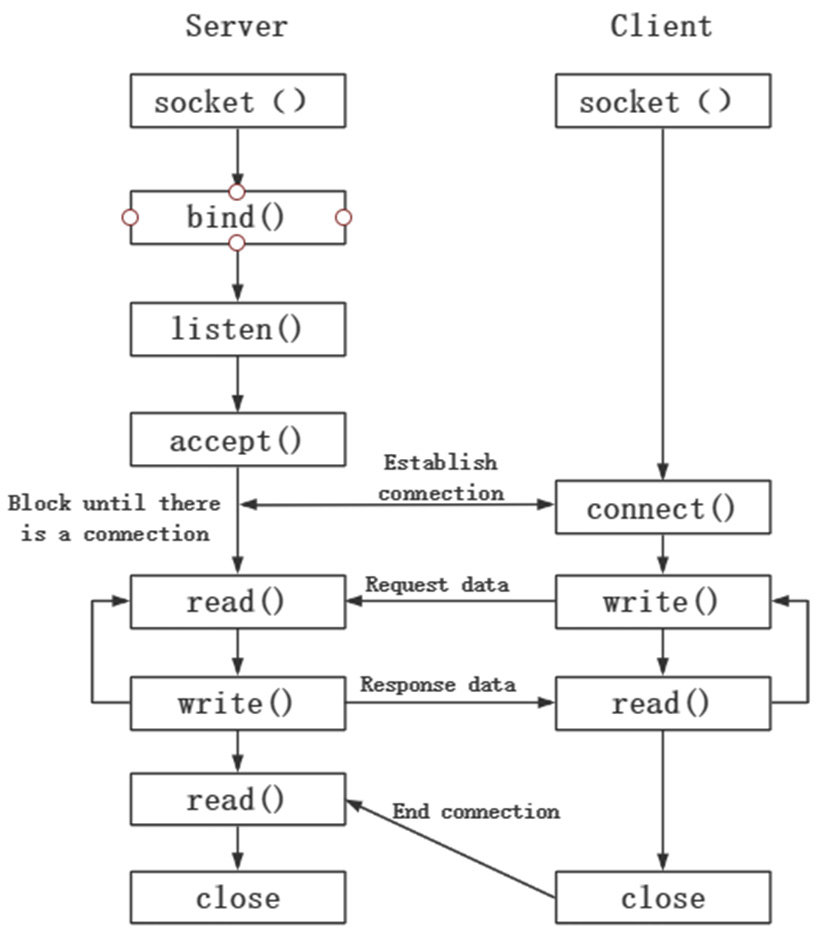
\includegraphics[width=1\textwidth]{Figure/Flow-chart-of-creating-a-socket-model.jpg}
    \caption{FTP design}
    \label{fig:ftp_des}
\end{figure}

\section{Systems organization}

\subsection{System architecture}
The system is built around a "Client-Server" architecture, where the "Client" initiates a connection and transfers a file to the "Server". The two main components of the system are the "Client" and the "Server", which communicate through a TCP connection. The following is a detailed breakdown of the system architecture:

\begin{itemize}
    \item Client: \begin{itemize}
        \item The client initiates the file transfer by establishing a TCP connection to the server.
        \item It first sends the file metadata (name and size), followed by the file data in chunks.
        \item The client waits for an acknowledgment (ACK) from the server after each chunk to ensure reliable data transfer.
        \item Once the entire file has been sent successfully, the client closes the connection.
    \end{itemize}

    \item Server: \begin{itemize}
        \item The server listens for incoming connections on a pre-defined port.
        \item Once the connection is established, it receives the file metadata and prepares to receive the file.
        \item The server receives the data from the file in chunks and writes the data to a file.
        \item After receiving each chunk, the server sends an acknowledgment (ACK) back to the client.
        \item When the file is fully received, the server signals the completion of the transfer and closes the connection.
    \end{itemize}
\end{itemize}

\thispagestyle{empty}
    \newpage

\subsection{Figure system organization}
\begin{figure}[ht!]
    \centering
    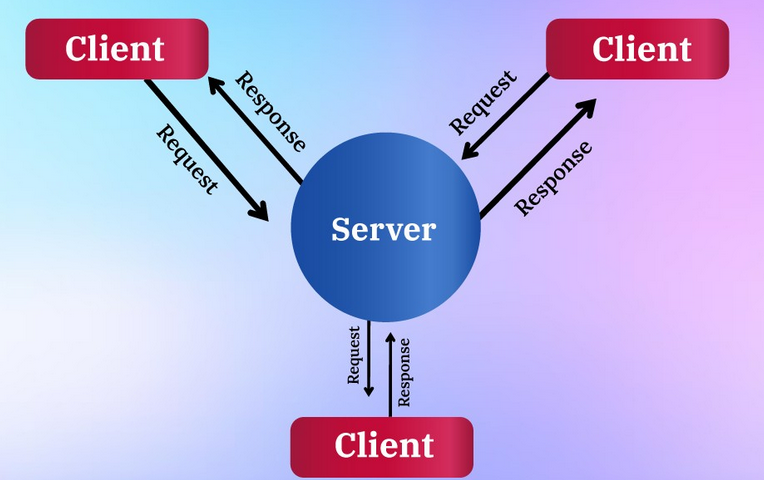
\includegraphics[width=1\textwidth]{Figure/System-architecture.png}
    \caption{System organization}
    \label{fig:system_organ}
\end{figure}

\section{File transfer implementation}

\subsection{Client code}
The following code snippet shows the implementation of the client in Python using TCP/IP for file transfer. The client connects to the server, sends the file metadata (name and size), and then transfers the file data in chunks. After sending each chunk, the client waits for an acknowledgment from the server before sending the next chunk.

\thispagestyle{empty}
    \newpage
    
\begin{lstlisting}[language=Python]
import socket
import os

def send_file():
    server_ip = '127.0.0.1'
    server_port = 21003
    filename = 'send.txt'

    try:
        with open(filename, 'rb') as file:
            client_socket = socket.socket(socket.AF_INET, socket.SOCK_STREAM)
            client_socket.connect((server_ip, server_port))
            
            file_name = os.path.basename(filename)
            file_size = os.path.getsize(filename)
            client_socket.send(f"{file_name},{file_size}".encode()) 

            ack = client_socket.recv(1024)
            print(f"Server acknowledgment: {ack.decode()}")

            while chunk := file.read(1024):
                client_socket.send(chunk)
                ack = client_socket.recv(1024)  
                print(f"Acknowledgment received: {ack.decode()}")

            print(f"File '{filename}' has been sent successfully")

    except Exception as e:
        print(f"Error: {e}")

    finally:
        client_socket.close()

if __name__ == "__main__":
    send_file()
\end{lstlisting}

\subsection{Server code}
The following code snippet shows the implementation of the server in Python using TCP/IP for file transfer. The server listens for incoming connections from the client, receives the file metadata (name and size), and then writes the received file data to disk in chunks. After receiving each chunk, the server sends an acknowledgment to the client.

\begin{lstlisting}[language=Python, caption=Server code for file transfer using TCP/IP]
import socket

def receive_file():
    server_ip = '0.0.0.0'  
    server_port = 21003
    allowed_ips = ['127.0.0.1', '192.168.48.140', '172.30.176.1'] 

    try:
        server_socket = socket.socket(socket.AF_INET, socket.SOCK_STREAM)
        server_socket.bind((server_ip, server_port))
        server_socket.listen(5) 

        print(f"Server is waiting for connection at {server_ip}:{server_port}...")

        while True: 
            client_socket, client_address = server_socket.accept()
            print(f"Connected to {client_address}")

            if client_address[0] not in allowed_ips:
                print(f"Connection from {client_address[0]} is not allowed.")
                client_socket.close()
                continue 

            file_info = client_socket.recv(1024).decode()
            filename, file_size = file_info.split(',')
            file_size = int(file_size)

            print(f"Receiving file: {filename} (Size: {file_size} bytes)")

            client_socket.send("Ready to receive file".encode())

            with open(f'received_{filename}', 'wb') as file:
                bytes_received = 0
                while bytes_received < file_size:
                    data = client_socket.recv(1024)
                    file.write(data)
                    bytes_received += len(data)

                    client_socket.send("ACK".encode())

            print(f"File '{filename}' received successfully and saved.")

            client_socket.close()

    except Exception as e:
        print(f"Error: {e}")

    finally:
        server_socket.close() 

if __name__ == "__main__":
    receive_file()

\end{lstlisting}

\subsection{Testing code snippet with myself}

\begin{figure}[h]
    \centering
    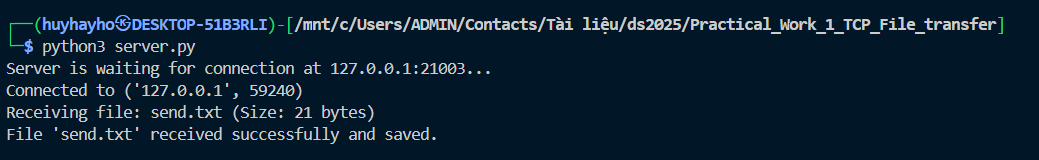
\includegraphics[width=1\linewidth]{Figure/server.png}
    \caption{Server command line}
    \label{fig:server_command_line}
\end{figure}

\begin{figure}[h]
    \centering
    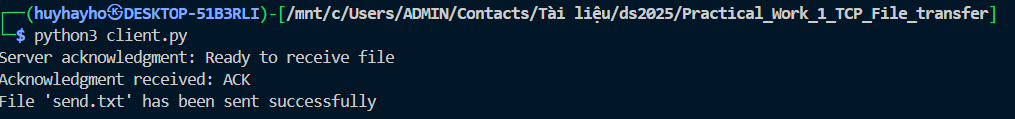
\includegraphics[width=1\linewidth]{Figure/Client.png}
    \caption{Client command line}
    \label{fig:client_command_line}
\end{figure}

\begin{figure}[h]
    \centering
    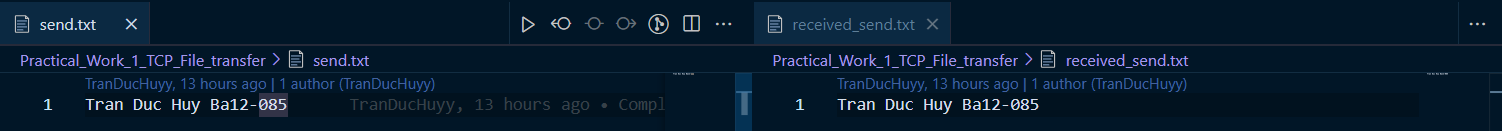
\includegraphics[width=1\linewidth]{Figure/Compare.png}
    \caption{Compare send.txt and received_send.txt}
    \label{fig:compare}
\end{figure}

\subsection{Testing code with groupmate}

\begin{figure}[h]
    \centering
    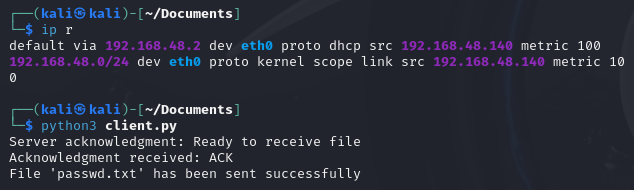
\includegraphics[width=1\linewidth]{Figure/crab241_client.png}
    \caption{Client command line - crab241 computer}
    \label{fig:client_command_line}
\end{figure}


\begin{figure}[h]
    \centering
    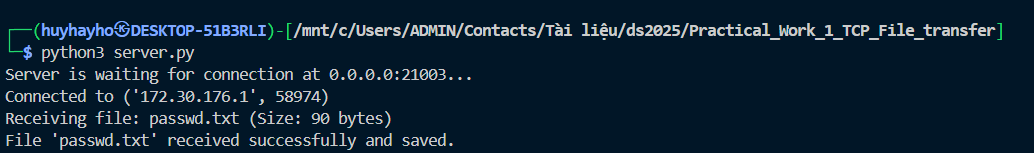
\includegraphics[width=1\linewidth]{Figure/huy_server.png}
    \caption{Server command line - my computer}
    \label{fig:server_command_line}
\end{figure}

\thispagestyle{empty}
    \newpage

\section{Conclusion}

In this project, we successfully implemented a file transfer system using the TCP/IP protocol, following a client-server architecture. The "Client" and "Server" components communicated efficiently through a socket connection, where the client sent a file in chunks and the server received the chunks and stored the file.

The key features of the system include:
\begin{itemize}
    \item Reliable file transfer with acknowledgment after each chunk.
    \item Handling of file metadata, such as the file's name and size, before the transfer begins.
    \item A clear separation of responsibilities between the client (sending the file) and the server (receiving and saving the file).
    \item Simple error handling to handle connection issues and ensure robust transfer.
\end{itemize}

In conclusion, this project provided a solid foundation for understanding how to implement a basic file transfer system using TCP/IP sockets, with practical insights into how such systems function and can be enhanced for real-world use.

\section{References}

\begin{thebibliography}{99}
    
    \bibitem{ref1} Mắt Bão. (n.d.). \textit{Socket là gì? Khái niệm cần biết về giao thức TCP/IP và UDP}. Retrieved from \url{https://wiki.matbao.net/socket-la-gi-khai-niem-can-biet-ve-giao-thuc-tcp-ip-va-udp/}
    
\end{thebibliography}

\end{document}
